\documentclass[14pt,dvipsnames]{extarticle}

\usepackage[T1]{fontenc}

\usepackage{microtype}
\DisableLigatures{encoding=*,family=razor}

\usepackage{url}
\usepackage{calc}
\usepackage{xspace}

\usepackage{lipsum}

\usepackage[pdftex]{graphicx}
\usepackage{pdfpages}

\usepackage{multicol}
\newenvironment{columns}
{\begin{multicols}{2}
%\@afterindentfalse%\@afterheading
}
{\end{multicols}
\ignorespacesafterend
}

\usepackage[dvipsnames]{colortbl}

\newcommand{\cfbox}[2]{%
    \colorlet{currentcolor}{.}%
    {\color{#1}%
    \fbox{\color{currentcolor}#2}}%
}

%%----------------------------------------------------------------------
%%-- Notes

\usepackage[many]{tcolorbox}

\newtcolorbox{recon}[1][]{
  colback=RedOrange!16,
  colframe=RedOrange,
  fonttitle=\bfseries,
  /tcb/fontupper=\it,
%  title=RECON+,
  #1}

%%----------------------------------------------------------------------
%%-- Font

\usepackage[scaled]{helvet}
\renewcommand*\familydefault{\sfdefault}

%%----------------------------------------------------------------------
%%-- Geometry

\usepackage[letterpaper, portrait, margin=0.5in, bottom=0.5in, footskip=0.25in]{geometry}

\setlength{\columnsep}{0.35in}

%\raggedcolumns

%%----------------------------------------------------------------------
%%-- Headers & Footers

%%----------------------------------------------------------------------
%%-- Sections

\usepackage{titlesec}
%\newcommand{\sectionbreak}{\clearpage}

%\titleformat{\section}[hang]
%  {\usefont{T1}{qhv}{b}{n}}
%  {}
%  {0em}
%  {\hspace{-0.4pt}\Large \thesection\hspace{0.6em}}

\titleformat{name=\section,numberless}[block]
  {\Large\usefont{T1}{razor}{m}{n}} % 
  {}
  {0pt}
  {\colorsection}

\newcommand{\pagetitle}[1]{%
  \clearpage
  \section{#1}
}

\newcommand{\colorsection}[1]{%
  \colorbox{CornflowerBlue}{\parbox{\dimexpr\textwidth-2\fboxsep}{\hspace{.375\baselineskip}\textcolor{White}{#1}\vspace{.25\baselineskip}}}}

\titleformat{name=\subsection,numberless}[block]
  {\large\usefont{T1}{razor}{m}{n}} % 
  {}
  {0pt}
  {\colorsubsection}

\newcommand{\colorsubsection}[1]{%
  \colorbox{CornflowerBlue!10}{\parbox{\dimexpr\textwidth-2\fboxsep}{\hspace{.375\baselineskip}\textcolor{CornflowerBlue}{#1}\vspace{.25\baselineskip}}}}

\titlespacing*{\section}
{0pt}% left margin
{8pt}% before
{0pt}% after

\titlespacing*{\subsection}
{0pt}% left margin
{0pt}% before
{-9pt}% after

\newcommand{\missionrule}[1]{\noindent\textbf{#1}\xspace}

%%----------------------------------------------------------------------
%%-- Lists

\newenvironment{squishitemize}
{\begin{list}{$\bullet$}{%
    \setlength{\itemsep}{2pt}%
    \setlength{\parsep}{2pt}%
    \setlength{\topsep}{2pt}%
    \setlength{\parskip}{0pt} %
%    \setlength{\labelwidth}{.5in}%
%    \setlength{\labelsep}{0.05in} %
%    \setlength{\leftmargin}{0.2in} %
    \renewcommand{\labelitemi}{--}}}
  {\end{list}}

%%----------------------------------------------------------------------
%%-- Paragraphs

\setlength{\parskip}{0.8\baselineskip}%

\newcommand{\reconplus}{\textbf{RECON+}\xspace}

\setcounter{secnumdepth}{0}

\usepackage[dotinlabels]{titletoc}

\titlecontents{section}[7mm]% [left]
    {\addvspace{-8pt}}% {above}
    {\bf\contentslabel{7mm}}% {before with label}
    {}% {before without label}
    {\bf\titlerule*[2.7mm]{.}\contentspage}% {filler and page}
    [\addvspace{0mm}]% [after]

\titlecontents{subsection} [17mm]
    {}
    {\contentslabel{10mm}}
    {}
    {\titlerule*[2.7mm]{.}\contentspage}

\titlecontents{subsubsection} [30mm]
    {}
    {\contentslabel{13mm}}
    {}
    {\titlerule*[2.7mm]{.}\contentspage}

\setcounter{tocdepth}{1}


\usepackage{multicol}
\usepackage{multirow}
\usepackage{amsmath}
\usepackage{tabularx}
\usepackage{array}
\newcolumntype{C}[1]{>{\centering\let\newline\\\arraybackslash\hspace{0pt}}m{#1}}
\newcolumntype{F}[1]{>{\centering\let\newline\\\arraybackslash\hspace{0pt}}p{#1}}
\newcolumntype{L}[1]{>{\raggedright\let\newline\\\arraybackslash\hspace{0pt}}m{#1}}
\newcolumntype{R}[1]{>{\raggedleft\let\newline\\\arraybackslash\hspace{0pt}}m{#1}}
\newcolumntype{E}[1]{>{\raggedright\let\newline\\\arraybackslash\hspace{0pt}}p{#1}}
\newcolumntype{R}[1]{>{\raggedleft\let\newline\\\arraybackslash\hspace{0pt}}m{#1}}
\newcolumntype{O}[1]{>{\raggedleft\let\newline\\\arraybackslash\hspace{0pt}}p{#1}}

\usepackage{latexsym}

\usepackage{fancyhdr}
\fancypagestyle{plain}{%
\fancyhf{}
\fancyfoot[C]{\footnotesize\usefont{T1}{razor}{m}{n}[~\thepage~]}
\fancyfoot[R]{\footnotesize\usefont{T1}{razor}{m}{n}[~RECON+~]}
\renewcommand{\headrulewidth}{0pt}
\renewcommand{\footrulewidth}{0pt}}
\pagestyle{plain}


\usepackage{eso-pic}

\newcommand\BackgroundPic[1]{%
\put(0,0){%
\parbox[b][\paperheight]{\paperwidth}{%
\vfill%
\centering%
\includegraphics[width=\paperwidth,height=\paperheight,keepaspectratio]{#1}%
\vfill%
}}}

\newcommand{\squelchbackground}{%
\ClearShipoutPicture
}

\newcommand{\restorebackground}{%
\setbackground
}
\newcommand{\setbackground}{%
\AddToShipoutPicture{\BackgroundPic{art/background/background.pdf}}%
}

%%----------------------------------------------------------------------
%%----------------------------------------------------------------------
\begin{document}
\thispagestyle{empty}
\includepdf[pages={1}]{art/cover/cover.pdf}

\clearpage

%\setbackground
\setcounter{page}{1}
\fancyfoot[L]{\footnotesize\usefont{T1}{razor}{m}{n}[~Introduction~]}

\begin{figure*}[t!]
  \centering
  
\includegraphics{art/cover/title.pdf}  
\end{figure*}

  
\noindent\reconplus is a set of unofficial firefight missions for Corvus Belli's
\emph{Infinity} miniatures games.  Based around 150pt games, they are
slightly larger than the official starter box missions but half the
points of a traditional 300pt game.  Although they make great stepping
stones to full size tournament play for beginners, they are also fun
and challenging tactical games for experienced players. The action is
fast, games are quick, different weapons and tactics have increased
emphasis, and hard choices have to be made in designing army lists.

This packet is an iteration and refinement of the original unofficial
RECON format by Guerilla Miniatures Games\footnote{Version~2.0
  (February 2017) available at \url{http://bit.ly/2pSYxBm}}, which in
turn derived from the official ITS missions.  A few ambiguities are
clarified, and a number of tweaks made to the rules and missions based
on community preferences developed playing this format frequently in
local casual tournaments.

\tableofcontents

\vfill

\hfill{\small[ \reconplus release \today ]}

\clearpage
\fancyfoot[L]{\footnotesize\usefont{T1}{razor}{m}{n}[~Rules~]}

\section{Squad Construction}

Players simultaneously select their army lists at the start of a match
after establishing their mission, opponent, play area, and classified
objectives (explained below).  In a tournament setting players may
construct two army lists chosen from the same faction (including
sectorial) to use throughout the event.  Select which list to use each
round after learning your mission, opponent, play area, and choosing a
classified objective.

\reconplus army lists are chosen according to the following rules:

\vspace{-1em}
\begin{itemize}
\item You may select up to at most~150 army points.
\item Normal rules for SWC, Remotes, etc., apply.
\item Models with troop classification Character that cost more
  than~35pts are not permitted.
%\item At most half of the models may be Impetuous or Extremely Impetuous.
\item Only one model with the Impetuous or Extremely Impetuous
  characteristics may be included per every~4 models.  The Frenzy
  characteristic is not limited.

\item Only one model with multiple wounds or structure, Symbiont
  Armor, or V: No Wound Incapacitation may be included per every~4
  models.
  
\item Only a single fireteam of any type may be included or active at
  any time.  It may contain a maximum of~3 members and may not be
  reformed to more than that.
\item The entire army list must be organized within a single combat
  group.
\end{itemize}

Players or event organizers may optionally also permit either or both
of the following:

\begin{squishitemize}
\item \emph{Spec-Ops:} You may include a single Spec-Ops troop of up to 12 XP.
\item \emph{Mercs:} All mercenaries may be selected regardless of normal
  faction restrictions.
\end{squishitemize}

All other standard \emph{Infinity}, \emph{Human Sphere}, and ITS rules
and FAQs apply.

\begin{recon}
  N.B.: The Impetuous restrictions here differ from those in the
  original RECON packet, and specific clarifications made on Symbiont
  Armor and No Wound Incapacitation.
  %(February~2017), which limits army lists to
%  a single such model.
\end{recon}

\clearpage
\section{Play Area}

\reconplus games take place in a play area~24'' wide and~30--36''
long, with 36'' long recommended but not critical.  Make sure to
measure the play area precisely before choosing classified objectives
or lists.  Player edges are the short ends of the play area.
Deployment zones are measured from those player edges as follows:

\bigskip
\centerline{
\begin{tabular}{cc}
  \rowcolor{CornflowerBlue}\textcolor{White}{\textbf{Play Area Length}} & \textcolor{White}{\textbf{Deployment Zone}}\\
  36'' & 6''\\
  \rowcolor{CornflowerBlue!10} 35'' & 5.5''\\
  34'' & 5''\\
  \rowcolor{CornflowerBlue!10} 33'' & 4.5''\\
\end{tabular}%
\quad\quad%
\begin{tabular}{cc}
  \rowcolor{CornflowerBlue}\textcolor{White}{\textbf{Play Area Length}} & \textcolor{White}{\textbf{Deployment Zone}}\\
  32'' & 4''\\
  \rowcolor{CornflowerBlue!10} 31'' & 3.5''\\
  30'' & 3''\\
  \\
\end{tabular}
}

Be sure to place terrain to minimize long firelanes.  At least one
piece of terrain should touch each play area edge to prevent open
spaces running its full length.  The tallest terrain should be toward
the middle of the play area, to prevent creating a ``sniper bowl.''

\begin{recon}
  Flexibility in length is motivated by Corvus Belli's starter set
  mats, which vary in length.
  % such as are included in
  % the \emph{Operation: Icestorm} and other starter sets.  These vary
  % in length but most are actually less than 36'' long.
\end{recon}

\section{Gameplay}

ITS rules are used except when overridden by these rules or missions.
The following rules apply in all \reconplus games unless noted
otherwise by a mission or event.

\subsection{Pregame}

Match preparation follows these rules.  They are no different from
starting an ITS game, but are included here for convenience and to
make clear they apply.

\missionrule{Startup Sequence.}  The following sequence is used in
setting up each match---

\begin{squishitemize}  
\item Establish mission, opponents \& factions, and play area.

\item Select classified objectives (see below).
  
\item Simultaneously reveal chosen army lists (the public information).

\item Initiative Roll.

\item Deployment, including HVTs (see below).
\end{squishitemize}

\missionrule{Classified Objectives.}  Before choosing their army list,
each player draws~2 classified objective cards and secretly chooses~1
to keep in play for themselves (do not reveal either).  Achieving
classified objectives, including the Secure HVT option (see below), is
worth~2 objective points in each \reconplus mission.  They may only be
scored once.

\missionrule{High Value Targets.}  Each player must deploy a High
Value Target~(HVT) model at the beginning of their deployment.  These
must be placed at least~4'' outside of both deployment zones, directly
on the play area itself (not on any terrain).  A player may opt at any
point to replace their chosen classified objective with the Secure HVT
classified objective:

\begin{squishitemize}
\item \textbf{Secure HVT} is accomplished if at game end the player
  has a troop not in a Null state inside the zone of control of the
  opposing player's HVT, while at the same time there are no enemy
  troops not in a Null state within the zone of control of their own
  HVT.
\end{squishitemize}

\subsection{In-Game}

The following in-game rules apply to each \reconplus mission.

\missionrule{Command Tokens: Strategic Use.}  The second player may
only nullify a single Regular Order from their opponent's order pool
at the beginning of the game.

%Command tokens may otherwise be used as normal, except a player may
%never have more than one active fireteam of any type.

\begin{recon}
  N.B.: The current original RECON packet prohibits
  Strategic Use of Command Tokens.
%  N.B.: The most recent original RECON packet completely prohibits
%  Strategic Use of Command Tokens, which \reconplus does not.
\end{recon}

\missionrule{Specialists.}  Hackers, Doctors, Engineers, Forward
Observers, Paramedics, and troops with the Chain of Command special
skill are considered Specialist Troops in all missions.  Repeaters and
G: Servants cannot be used to perform tasks reserved for Specialist
Troops.

\missionrule{Exclusion Zone.}  Some missions include an Exclusion Zone
in the play area configuration.  Troops may not use Airborne
Deployment, Forward Deployment, Mechanized Deployment, Infiltration
special skills, or the deployment rule of the Impersonation special
skill to deploy within an Exclusion Zone.  Troops that suffer
Dispersion are not affected by Exclusion Zones.

\missionrule{Hack Mission Objective.} Some missions make the following
short skill available.

{\setlength\fboxrule{2pt}
\cfbox{LimeGreen}{\begin{minipage}{6.5in}
  \colorbox{LimeGreen}{\parbox{\linewidth-2\fboxsep}{\textcolor{White}{\textbf{\large Hack Mission Objective} \hfill Short Skill}}}\\
  \colorbox{SkyBlue}{\parbox{\linewidth-2\fboxsep}{\textcolor{White}{Attack}}}

  \medskip
  \textsc{Requirements}
  \begin{squishitemize}
  \item The user must be a Specialist Troop model (not a marker) in
    base contact with an Antenna or Console.
  \end{squishitemize}

  \medskip
  \colorbox{Gray!24}{\begin{minipage}{\linewidth-2\fboxsep}

  \medskip      
      \textsc{Effects}
      \begin{squishitemize}
      \item The user makes a Normal WIP roll to hack an Antenna or
        Console in base contact.  Hackers receive a +3 MOD on this
        roll.

      \item If successful, the acting player takes control of the
        Antenna or Console (mark it appropriately).  The other player
        loses control of that mission element if they had previously
        hacked it (remove any such marker).
        
%      \item This skill may be invoked as many times as desired if the
%        user continues to fail.
      \end{squishitemize}
    \end{minipage}}
\end{minipage}}}

\subsection{Endgame}

The following rules outline end game conditions for \reconplus
missions.

\missionrule{End Game.}  Before any lists are constructed, players or
event organizers must select one of the following end game conditions
to apply to all missions:

\vspace{-1em}
\begin{itemize}
\item \textbf{RECON+:} All matches end after~3 game turns or the time
  limit (see below) is reached.  Unless noted otherwise by a mission,
  \emph{Retreat!} rules apply as given in the main \emph{Infinity}
  rulebook except the game does not end once one player has no models
  in play.  The remaining player may play out the game turns
  attempting to score objectives.

\item \textbf{ITS:} All matches end after~3 game turns or the time
  limit (see below) is reached.  \emph{Retreat!} rules apply unless
  noted otherwise by a mission.  The match ends at the conclusion of
  the current game turn if either player is eliminated or starts their
  active turn in a \emph{Retreat!} situation (which requires
  \emph{Retreat!} rules to be in play for the mission).
\end{itemize}

\vspace{-1em}
\begin{recon}
  The \reconplus end game conditions avoid creating an awkward
  disincentive in which players want to destroy their opponent's
  models, but not so quickly as to make the game end before they
  themselves can capture objectives.  However, almost all tournaments
  use the ITS end game conditions and players hoping to compete in
  such should be familiar with the peculiar strategic considerations
  those rules create.
\end{recon}

% In addition, unless the mission notes otherwise, if one of the players
% starts their active turn in a \emph{Retreat!} situation, then the
% match will end with the conclusion of the game turn.

\missionrule{Time Limit.} Matches in organized play run for~75 minutes
unless announced otherwise.  Event organizer(s) must make clear
beforehand how this will be enforced, with either an immediate hard
stop or permitting the current player or even game turn to be
completed.

\begin{recon}
  For beginner and casual events the time limit should be loose, with
  time reserved in the schedule (e.g.,~90 minute rounds) for matches
  to finish out their final game turn.
\end{recon}

\missionrule{Destroyed.} Models are considered destroyed when they
enter the Dead state, are in a Null state at the end of the game, or
have not been deployed by the end of the game.  Those models not
destroyed are considered to have survived, as are models in
\emph{Retreat!} which exit the play area through the long edge of
their player's deployment zone.

\subsection{Scoring}

\missionrule{Scoring.}  All \reconplus missions are scored out of a
possible~9 objective points.  Players do NOT automatically receive
maximum points for eliminating their opponent.
  
\begin{recon}
  If your opponent cripples your ability to achieve the mission
  objectives before you eliminate them, then you have not actually
  earned a full victory!
\end{recon}

\missionrule{Domination.}  A player dominates a Sector, as defined by
some missions, if their models within that Sector comprise more army
points than those of their opponent.  Models are considered to be
solely within the single Sector, if any, containing more than half
their base.  Only troops not in a Null state, markers representing
troops, AI Beacons, Proxies, and G: Servant models are counted.
Troops possessing the Shasvastii special skill are also counted when
in the Spawn Embryo or any non-Null state.  The extra army points
provided by Baggage equipment possessed by troops not in a Null state
are also counted.

%\clearpage
\section{Mission Elements}

Most \reconplus missions revolve around interacting with elements of
the \emph{Infinity} world as defined in each scenario.  These elements
may be represented by a physical 3D piece or a marker as is
convenient.  In either case they are considered to have the
silhouettes given below and provide cover or block LOF accordingly,
except Civilians, which do neither.

\begin{recon}
  This is a slight variance from the main \emph{Infinity} rulebook, in
  which mission elements such as objectives only grant cover when
  physically represented by 3D terrain pieces.
\end{recon}

Mission elements cannot be directly targeted by attacks other than
those provided by the mission, but can be affected by attacks through
dispersion and other mechanics.  Any player that damages a mission
element automatically loses the match at its conclusion and grants
their opponent~2 objective points (within the maximum of~9).

\bigskip
\centerline{
\begin{tabular}{cccccc}
  \rowcolor{CornflowerBlue}\textcolor{White}{\textbf{Element}} & \textcolor{White}{\textbf{Type}} & \textcolor{White}{\textbf{ARM}} & \textcolor{White}{\textbf{BTS}} & \textcolor{White}{\textbf{W/STR}} & \textcolor{White}{\textbf{Silhouette}} \\
  Antenna & Scenery Item & 4 & 3 & 2 & S6~ (40mm base x 55mm high)\\
  \rowcolor{CornflowerBlue!10} Console & Scenery Item & 0 & 0 & 1 & S5~ (40mm base x 45mm high)\\
  Civilian & Neutral Model & 0 & 0 & 1 & S1- (20mm base x 25mm high)\\
  \rowcolor{CornflowerBlue!10} HVT & Neutral Model & 0 & 0 & 1 & S2~ (25mm base x 40mm high)\\
  Tech-Coffin & Scenery Item & 1 & 0 & 1 & S5~ (40mm base x 45mm high)\\
\end{tabular}
}

\begin{recon}
  Civilians have a 20mm base here to denote them as diminutive,
  cowering, and not cover (by \emph{Human Sphere} they do not block
  LOF).  Feel free to use 25mm bases/markers.
\end{recon}

%\section{Materials}
%
%As always, for an organized event, players should bring:
%\begin{squishitemize}
%\item Two printed copies of your complete army lists, for yourself and
%  the event organizer(s).

%\item Printed copies of your courtesy army lists to give to your
%  opponent each round.
%
%\item All models, dice, markers, templates, and other materials needed
%  to play.
%\end{squishitemize}

\vfill
\centerline{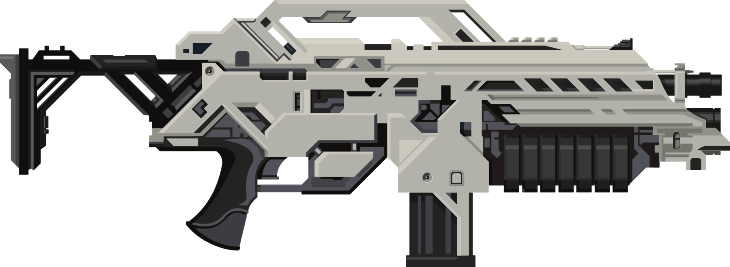
\includegraphics[width=0.5\linewidth]{art/rifle.pdf}}
%\vfill
\vbox to 0pt{}

\clearpage
\fancyfoot[L]{\footnotesize\usefont{T1}{razor}{m}{n}[~\rightmark~]}

%%----------------------------------------------------------------------
\pagetitle{Mission: Annihilate}
\label{mission:annihilation}

\subsection{Play Area Configuration}

There is no special play area configuration for this mission.

\subsection{Mission Rules}

There are no special gameplay rules for this mission.

\subsection{End Game}

\emph{Retreat!} rules DO NOT apply in this mission.

\subsection{Scoring}

\noindent%
\begin{tabular}{L{5.85in}C{0.5in}C{0.25in}C{0.25in}}
    \rowcolor{CornflowerBlue} & \textcolor{White}{\textbf{Obj.}} & \multicolumn{2}{c}{\textcolor{White}{\textbf{Player}}}\\
  \rowcolor{CornflowerBlue}\textcolor{White}{\textbf{Condition}} &
                                                                   \textcolor{White}{\textbf{Pts}} & \textcolor{White}{\textbf{1}} & \textcolor{White}{\textbf{2}} \\
  %%
  %% ----------------------------------------------
  At least 25pts of opponent's army list destroyed at game end. & 1 & $\Box$ & $\Box$ \\
  \rowcolor{CornflowerBlue!10} At least 50pts of opponent's army list destroyed at game end. & 1 & $\Box$ & $\Box$ \\
  At least 75pts of opponent's army list destroyed at game end. & 1 & $\Box$ & $\Box$ \\
  \\[-9pt]
  \rowcolor{CornflowerBlue!10} At least 25pts of player's army list survived at game end. & 1 & $\Box$ & $\Box$ \\
  At least 50pts of player's army list survived at game end.& 1 & $\Box$ & $\Box$ \\
  \rowcolor{CornflowerBlue!10} At least 75pts of player's army list survived at game end. & 1 & $\Box$ & $\Box$ \\
  \\[-9pt]
  More points of opponent's army list destroyed at game end. & 1 & $\Box$ & $\Box$ \\
  %%
  %% ----------------------------------------------
  \\[-9pt]  
  \rowcolor{CornflowerBlue!10} Classified objective achieved. & 2 & $\Box$ & $\Box$ \\
  \\
\multicolumn{2}{r}{\textbf{Sum:}} & $\rule{0.25in}{0.15mm}$ & $\rule{0.25in}{0.15mm}$\\
\end{tabular}


%%----------------------------------------------------------------------
\pagetitle{Mission: Break Through}
\label{mission:frontline}

\subsection{Play Area Configuration}

There is no special play area configuration for this mission.

\subsection{Mission Rules}

There are no special gameplay rules for this mission.

\subsection{End Game}

\emph{Retreat!} rules DO NOT apply in this mission.

%There are no special end game conditions for this mission.

\subsection{Scoring}

% The following rules determine the outcome of this mission---

\missionrule{Sectors.}  At game end, measure out three Sectors on the
play area each covering the full extent between its long edges:

\begin{squishitemize}
\item One central Sector extending~4'' on both sides of the short
  centerline.
\item Sectors covering the~8'' beyond the central sector toward the
  player edges.
\end{squishitemize}

%Troops in a null state, other markers (such as deployable equipment),
%fake Holoechoes, and other elements are not counted.

\noindent%
\begin{tabular}{L{5.85in}C{0.5in}C{0.25in}C{0.25in}}
    \rowcolor{CornflowerBlue} & \textcolor{White}{\textbf{Obj.}} & \multicolumn{2}{c}{\textcolor{White}{\textbf{Player}}}\\
  \rowcolor{CornflowerBlue}\textcolor{White}{\textbf{Condition}} &
                                                                   \textcolor{White}{\textbf{Pts}} & \textcolor{White}{\textbf{1}} & \textcolor{White}{\textbf{2}} \\
  %%
  %% ----------------------------------------------
  Dominate the Sector farthest from your deployment zone. & 4 & $\Box$ & $\Box$ \\
  \rowcolor{CornflowerBlue!10} Dominate the Sector at the center of the play area. & 2 & $\Box$ & $\Box$ \\
  Dominate the Sector closest to your deployment zone. & 1 & $\Box$ & $\Box$ \\
  %%
  %% ----------------------------------------------
  \\[-9pt]  
  \rowcolor{CornflowerBlue!10} Classified objective achieved. & 2 & $\Box$ & $\Box$ \\
  \\
\multicolumn{2}{r}{\textbf{Sum:}} & $\rule{0.25in}{0.15mm}$ & $\rule{0.25in}{0.15mm}$\\
\end{tabular}


%%----------------------------------------------------------------------
\pagetitle{Mission: Exfiltrate}
\label{mission:exfiltrate}

\subsection{Play Area Configuration}

As part of their army deployment, before placing their HVT, each
player deploys~4 Civilian models inside the half of the Exclusion Zone
(see below) on their opponent's side of the play area.  Civilians must
be placed at least~4'' away from all other Civilians.  They cannot be
placed on any terrain requiring a Climb entire order to reach.  No
model or marker may be deployed in base contact with any Civilian or
vice versa.

Once deployed, take~2 Agent and~2 Citizen importance markers (or
suitable proxies indistinguishable on the back side).  Turn them face
down, shuffle them, and randomly assign one to each of your Civilians
without being revealed to you or your opponent.

\missionrule{Exclusion Zone.}  There is an Exclusion Zone
extending~6'' on both sides of the short centerline of the play area
(12'' long total) and covering the full extent between long edges.

\subsection{Mission Rules}

The Interrogate Civilian common skill on the following page is
available in this mission.

Once a Civilian has been revealed as an Agent, it may be directly
targeted by the opposing player as an enemy troop and no penalty is
incurred by them for damaging it.

% The Synchronize Civilian common skill cannot be applied to the
% Civilians in this mission.  Instead the following Common Skill is
% available.

\subsection{End Game}

There are no special end game conditions for this mission.
%(\emph{Retreat!} applies).

\subsection{Scoring}

\missionrule{Exfiltrated.}  An Agent has been Exfiltrated if it is
wholly inside its player's deployment zone.

\missionrule{Secured.}  An Agent is Secured if it is wholly outside
the Exclusion Zone on its player's side of the play area.  An
Exfiltrated Agent is necessarily Secured, but not vice versa.

{\setlength\fboxrule{2pt}
\cfbox{CornflowerBlue}{\begin{minipage}{6.5in}
  \colorbox{CornflowerBlue}{\parbox{\linewidth-2\fboxsep}{\textcolor{White}{\textbf{\large Interrogate Civilian} \hfill Short Movement Skill}}}\\
  \colorbox{SkyBlue}{\parbox{\linewidth-2\fboxsep}{\textcolor{White}{Attack}}}

  \medskip
  \textsc{Requirements}
  \begin{squishitemize}
  \item The user must be a model (not a marker) in base contact with a
    Civilian deployed by their player.

  \item The user cannot already be in CivEvac state with a Civilian,
    unless it possesses the Doctor, Paramedic, or Chain of Command
    special skills, in which case it cannot already be in CivEvac
    state with~2 Civilians.

  \item The user cannot be Impetuous or Extremely Impetuous, including
    through the Frenzy characteristic having triggered.

  \item The user cannot possess the G: Servant or G: Synchronized
    special skills, or its Type of Troop be REM.
    
  \item The user cannot be part of a fireteam of any kind, and this
    short skill cannot be performed as part of a coordinated order.
    
%  \item The targeted Civilian cannot be in the CivEvac state with an
%    enemy model.
  \end{squishitemize}

  \medskip
  \colorbox{Gray!24}{\begin{minipage}{\linewidth-2\fboxsep}

  \medskip      
      \textsc{Effects}
      \begin{squishitemize}
      \item The user makes a Normal WIP roll to synchronize a
        designated Civilian in base contact that was placed by their
        player.  Doctors and Paramedics receive a +3 MOD on this roll.
        Models from the Tohaa or Combined Army factions (including any
        sectorial) suffer a -3 MOD.

      \item If the roll is successful, the Civilian's importance
        marker is revealed to both players if it has not already.  If,
        and only if, the Civilian is an Agent, it enters the CivEvac
        state with the user (\emph{Human Sphere}, page~95).

      \item If the roll fails, the opposing player moves the Civilian
        as far as possible following general movement rules up to 2''
        from the user.
      \end{squishitemize}
    \end{minipage}}
\end{minipage}}}

\vspace*{-5pt}

\noindent%
\begin{tabular}{L{5.85in}C{0.5in}C{0.25in}C{0.25in}}
    \rowcolor{CornflowerBlue} & \textcolor{White}{\textbf{Obj.}} & \multicolumn{2}{c}{\textcolor{White}{\textbf{Player}}}\\
  \rowcolor{CornflowerBlue}\textcolor{White}{\textbf{Condition}} &
                                                                   \textcolor{White}{\textbf{Pts}} & \textcolor{White}{\textbf{1}} & \textcolor{White}{\textbf{2}} \\
  %%
  %% ----------------------------------------------
  Have at least one of your Agents in CivEvac state at game end. & 1 & $\Box$ & $\Box$ \\
  \rowcolor{CornflowerBlue!10} Have both of your Agents in CivEvac state at game end. & 1 & $\Box$ & $\Box$ \\
  \\[-9pt]
  Have at least one of your Agents Secured at game end. & 1 & $\Box$ & $\Box$ \\
  \rowcolor{CornflowerBlue!10} Have both of your Agents Secured at game end. & 1 & $\Box$ & $\Box$ \\
  \\[-9pt]  
  Have at least one of your Agents Exfiltrated at game end. & 1 & $\Box$ & $\Box$ \\
  \rowcolor{CornflowerBlue!10} Have both of your Agents Exfiltrated at game end. & 1 & $\Box$ & $\Box$ \\
  \\[-9pt]
  Have more Agents in CivEvac state at game end than your opponent. & 1 & $\Box$ & $\Box$ \\
  %%
  %% ----------------------------------------------
  \\[-9pt]  
  \rowcolor{CornflowerBlue!10} Classified objective achieved. & 2 & $\Box$ & $\Box$ \\
  \\
\multicolumn{2}{r}{\textbf{Sum:}} & $\rule{0.25in}{0.15mm}$ & $\rule{0.25in}{0.15mm}$\\
\end{tabular}

%%----------------------------------------------------------------------
\pagetitle{Mission: Seize the Antennas}
\label{mission:seizetheantennas}

\subsection{Play Area Configuration}

Place one Antenna at the center of the play area and two more
each~10'' from the center on the long centerline toward the deployment
zones (2'' outside the deployment zones).  No model or marker may be
deployed in base contact with an Antenna.

%\begin{recon}
%  In the original RECON packet the outer Antennas are placed 12'' from
%  the center, thus partially within the deployment zones.
%\end{recon}

\subsection{Mission Rules}

The Hack Mission Objective short skill is available in this scenario
(see page~\pageref{sec:hack-objective}).

\subsection{End Game}

There are no special end game conditions for this mission.
%(\emph{Retreat!} applies).

\subsection{Scoring}

The following scoring conditions are evaluated at game end.

\noindent%
\begin{tabular}{L{5.85in}C{0.5in}C{0.25in}C{0.25in}}
    \rowcolor{CornflowerBlue} & \textcolor{White}{\textbf{Obj.}} & \multicolumn{2}{c}{\textcolor{White}{\textbf{Player}}}\\
  \rowcolor{CornflowerBlue}\textcolor{White}{\textbf{Condition}} &
                                                                   \textcolor{White}{\textbf{Pts}} & \textcolor{White}{\textbf{1}} & \textcolor{White}{\textbf{2}} \\
  %%
  %% ----------------------------------------------
  Connected to the Antenna closest to your deployment zone. & 1 & $\Box$ & $\Box$ \\
  \rowcolor{CornflowerBlue!10} Connected to the Antenna at the center of the play area. & 2 & $\Box$ & $\Box$ \\
  Connected to the Antenna farthest from your deployment zone. & 4 & $\Box$ & $\Box$ \\
  %%
  %% ----------------------------------------------
  \\[-9pt]  
  \rowcolor{CornflowerBlue!10} Classified objective achieved. & 2 & $\Box$ & $\Box$ \\
  \\
\multicolumn{2}{r}{\textbf{Sum:}} & $\rule{0.25in}{0.15mm}$ & $\rule{0.25in}{0.15mm}$\\
\end{tabular}


%%----------------------------------------------------------------------
\pagetitle{Mission: Smash and Grab}
\label{mission:smashandgrab}

\subsection{Play Area Configuration}

Place two Tech-Coffins, each equipped with a Datacube, on the short
centerline of the play area and each 5'' from the center toward a
different long edge (10'' apart).

\missionrule{Exclusion Zone.}  There is an Exclusion Zone
extending~6'' on both sides of the short centerline of the play area
(12'' long total) and covering the full extent between long edges.

\subsection{Mission Rules}

%\missionrule{Smash and Grab}
The following short skills and equipment are available in this mission.

\medskip
\centerline{\setlength\fboxrule{2pt}
\cfbox{LimeGreen}{\begin{minipage}{6.5in}
  \colorbox{LimeGreen}{\parbox{\linewidth-2\fboxsep}{\textcolor{White}{\textbf{\large Smash Tech-Coffin} \hfill Short Skill}}}\\
  \colorbox{SkyBlue}{\parbox{\linewidth-2\fboxsep}{\textcolor{White}{Attack}}}

  \medskip
  \textsc{Requirements}
  \begin{squishitemize}
  \item The user must be a Specialist Troop model (not a marker) in
    base contact with a Tech-Coffin equipped with a Datacube.

%  \item The user must not already be equipped with a Datacube, or, if
%    it also possesses Baggage equipment, must not be equipped with two
%    Datacubes.
  \end{squishitemize}

  \medskip
  \colorbox{Gray!24}{\begin{minipage}{\linewidth-2\fboxsep}

  \medskip
      \textsc{Effects}
      \begin{squishitemize}
%      \item Allows the user to make a Normal WIP roll to break the
%        Tech-Coffin's protections and extract the Datacube.  Hackers
%        receive a +3 MOD.

      \item The user makes a Normal WIP roll to extract the Datacube.
      Doctors and Paramedics receive~+3MOD and~+1B on this WIP check.

      \item If passed, the Tech-Coffin unequips a Datacube and
        the user equips it. % (or an additional
        %Datacube if it possesses Baggage and was already equipped with
        %one).

%      \item This skill may be invoked as many times as desired if the
%        user continues to fail.
      \end{squishitemize}
    \end{minipage}}
\end{minipage}}}

\medskip
\centerline{\setlength\fboxrule{2pt}
\cfbox{LimeGreen}{\begin{minipage}{6.5in}
  \colorbox{LimeGreen}{\parbox{\linewidth-2\fboxsep}{\textcolor{White}{\textbf{\large Grab Datacube} \hfill Short Skill}}}\\
  \colorbox{SkyBlue}{\parbox{\linewidth-2\fboxsep}{\textcolor{White}{Attack}}}

  \medskip
  \textsc{Requirements}
  \begin{squishitemize}
  \item The user must be a model (not a marker) in base contact with a
    a Datacube marker or a friendly troop equipped with a Datacube.
    Note that the user does NOT have to be a Specialist Troop to
    execute this skill.

%  \item The user must not already be equipped with a Datacube, or, if
%    it also possesses Baggage equipment, must not be equipped with two
%    Datacubes.
  \end{squishitemize}

  \medskip
  \colorbox{Gray!24}{\begin{minipage}{\linewidth-2\fboxsep}

      \medskip
      \textsc{Effects}
      \begin{squishitemize}
      \item The user designates a Datacube marker or a friendly model
        equipped with a Datacube in base contact from which to grab a
        Datacube.

%      \item The user automatically equips a Datacube (or an additional
%        Datacube if it possesses Baggage and was already equipped with
%        one).

      \item If a friendly troop was designated, it unequips a
        Datacube.  If a Datacube marker was designated, it is removed
        from play.

      \item The user automatically equips the Datacube.
      \end{squishitemize}
  \end{minipage}}
\end{minipage}}}

\centerline{\setlength\fboxrule{2pt}
\cfbox{LimeGreen}{\begin{minipage}{6.5in}
  \colorbox{LimeGreen}{\parbox{\linewidth-2\fboxsep}{\textcolor{White}{\textbf{\large Drop Datacube} \hfill Short Skill, ARO}}}\\
  \colorbox{SkyBlue}{\parbox{\linewidth-2\fboxsep}{\textcolor{White}{Attack}}}

  \medskip
  \textsc{Requirements}
  \begin{squishitemize}
  \item The user must be equipped with a Datacube.
  \end{squishitemize}

  \medskip
  \colorbox{Gray!24}{\begin{minipage}{\linewidth-2\fboxsep}

      \medskip
      \textsc{Effects}
      \begin{squishitemize}
%      \item By spending a short skill or ARO, the user automatically
%        unequips one Datacube.  Its player places a Datacube marker in
%        base contact with the model or at any point in its movement if
%        it made any.
      \item The user automatically unequips one Datacube.  Place a
        Datacube marker in base contact or at any point in the model's
        movement.
      \end{squishitemize}
  \end{minipage}}
\end{minipage}}}

\medskip
\centerline{\setlength\fboxrule{2pt}
\cfbox{Black}{\begin{minipage}{6.5in}
  \colorbox{Black}{\parbox{\linewidth-2\fboxsep}{\textcolor{White}{\textbf{\large Datacube} \hfill Automatic Equipment}}}\\
  \colorbox{White}{\parbox{\linewidth-2\fboxsep}{Obligatory}}

  \medskip
  \textsc{Requirements}
  \begin{squishitemize}
  \item A model cannot ever be equipped with more than one Datacube,
    unless it also possesses Baggage equipment, in which case it may
    equip two.
  \end{squishitemize}

  \medskip
  \colorbox{Gray!24}{\begin{minipage}{\linewidth-2\fboxsep}

      \medskip
      \textsc{Effects}
      \begin{squishitemize}
%      \item No model may ever be equipped with more than one Datacube,
%        unless it also possesses Baggage equipment, in which case it
%        may be equipped with two Datacubes.

      \item Immediately upon the user entering a Null state (e.g.,
        going Unconscious), their model being replaced with a marker
        (e.g., returning to the Camouflaged state), or being removed
        from the game (e.g., becoming Dead), they unequip the Datacube
        and a Datacube marker is placed by their player in base
        contact with the user or its former position.

        %If they possessed multiple Datacubes, a Datacube marker is
        %placed for each.
      \end{squishitemize}
  \end{minipage}}
\end{minipage}}}

\subsection{End Game}

There are no special end game conditions for this mission.
%(\emph{Retreat!} applies).

\subsection{Scoring}

\missionrule{Hold.} Players hold a Datacube whenever any of
their models are equipped with such.

\vspace*{-1pt}

\noindent%
\begin{tabular}{L{5.85in}C{0.5in}C{0.25in}C{0.25in}}
    \rowcolor{CornflowerBlue} & \textcolor{White}{\textbf{Obj.}} & \multicolumn{2}{c}{\textcolor{White}{\textbf{Player}}}\\
  \rowcolor{CornflowerBlue}\textcolor{White}{\textbf{Condition}} &
                                                                   \textcolor{White}{\textbf{Pts}} & \textcolor{White}{\textbf{1}} & \textcolor{White}{\textbf{2}} \\
  %%
  %% ----------------------------------------------
  Hold any Datacube at the end of game round~1. & 1 & $\Box$ & $\Box$ \\
  \rowcolor{CornflowerBlue!10} Hold any Datacube at the end of game round~2. & 1 & $\Box$ & $\Box$ \\
  Hold any Datacube at the end of game round~3. & 3 & $\Box$ & $\Box$ \\
  \\[-9pt]
  \rowcolor{CornflowerBlue!10} Hold any Datacube at any point throughout the game. & 1 & $\Box$ & $\Box$ \\
  \\[-9pt]
  Hold both Datacubes at the end of the game. & 1 & $\Box$ & $\Box$ \\
  %%
  %% ----------------------------------------------
  \\
\multicolumn{2}{r}{\textbf{Sum:}} & $\rule{0.25in}{0.15mm}$ & $\rule{0.25in}{0.15mm}$\\
\end{tabular}


%%----------------------------------------------------------------------
\pagetitle{Mission: Sweep and Clear}
\label{mission:sweepandclear}

\subsection{Play Area Configuration}

Place~2 Consoles, each 12'' from the play area long edges and 6'' from
the center toward the deployment zones.  No model or marker may be
deployed in base contact with a Console.

\subsection{Mission Rules}

The Connect Mission Objective short skill may be used on the Consoles
in this scenario (see page~\pageref{sec:hack-objective}).  Engineers
receive a~+3 MOD on the WIP check to connect a Console.

\subsection{End Game}

There are no special end game conditions for this mission.

\subsection{Scoring}

% The following rules determine the outcome of this mission---

\missionrule{Sectors.}  After each game round measure four
Sectors on the play area dividing the space between the deployment
zones into equal quarters and determine Domination of each.

\missionrule{Search Teams.} Forward Observers not in a Null state
provide an additional~4 victory points toward Domination in this
mission.  Troopers with the Sensor special skill and not in a Null
state provide an additional~8 victory points toward Domination in this
mission. These bonuses apply cumulatively for troopers that possess
both skills.

\missionrule{Tapped Sensor Grid.}  After each game round, for each
Console they have currently connected and a model (not a marker) in
base contact, players may designate a Sector in which they are
considered to have an additional~20 army points for purposes of
Domination.  Both players make this declaration simultaneously.  A
single Sector may be designated twice by a player if they are able to
use both Consoles.

\noindent%
\begin{tabular}{L{5.85in}C{0.5in}C{0.25in}C{0.25in}}
    \rowcolor{CornflowerBlue} & \textcolor{White}{\textbf{Obj.}} & \multicolumn{2}{c}{\textcolor{White}{\textbf{Player}}}\\
  \rowcolor{CornflowerBlue}\textcolor{White}{\textbf{Condition}} &
                                                                   \textcolor{White}{\textbf{Pts}} & \textcolor{White}{\textbf{1}} & \textcolor{White}{\textbf{2}} \\
  %%
  %% ----------------------------------------------
  Dominate more Sectors following game round~1. & 1 & $\Box$ & $\Box$ \\
  \rowcolor{CornflowerBlue!10} Dominate more Sectors following game round~2. & 2 & $\Box$ & $\Box$ \\
  Dominate more Sectors following game round~3. & 3 & $\Box$ & $\Box$ \\
  \\[-9pt]
  \rowcolor{CornflowerBlue!10} Have more Consoles connected at game end. & 1 & $\Box$ & $\Box$ \\
  %%
  %% ----------------------------------------------
  \\
\multicolumn{2}{r}{\textbf{Sum:}} & $\rule{0.25in}{0.15mm}$ & $\rule{0.25in}{0.15mm}$\\
\end{tabular}


\clearpage
\section{Reference Guides}

\subsection{Random Mission Table}
\bigskip
\centerline{
\begin{tabular}{C{0.75in}C{1.75in}C{0.5in}C{1.25in}L{2in}}
  \rowcolor{CornflowerBlue}\textcolor{White}{\textbf{D20}} & \textcolor{White}{\textbf{Mission}} & \textcolor{White}{\textbf{Page}} & \textcolor{White}{\textbf{Elements}} & \textcolor{White}{\textbf{Description}}\\
  1--4 & Annihilate & \pageref{mission:annihilation} & - & Kill them all.\\
  \rowcolor{CornflowerBlue!10} 5--7 & Break Through & \pageref{mission:frontline} & - & Puncture the frontline.\\
  8--10 & Exfiltrate & \pageref{mission:exfiltrate} & 8 Civilians & Extract your agents.\\
  \rowcolor{CornflowerBlue!10} 11--14  & Seize the Antennas & \pageref{mission:seizetheantennas} & 3 Antennas & Control the transmitters.\\
  15--17 & Smash and Grab & \pageref{mission:smashandgrab} & 2 Tech-Coffins & Steal the data.\\
  \rowcolor{CornflowerBlue!10} 18--20 & Sweep and Clear & \pageref{mission:sweepandclear} & 2 Consoles & Search the area.\\
\end{tabular}
}

\bigskip
\centerline{\textit{Seize the Antennas or Annihilate are recommended for introductory games.}}

\vspace{-0.5em}
\subsection{Play Area Configurations}

\hfill
\begin{minipage}{2in}\centering
\colorbox{CornflowerBlue}{\parbox[t][12pt]{\linewidth-2\fboxsep}{\centering\textcolor{White}{\textbf{Annihilate}}}}

\smallskip
\includegraphics[scale=0.9]{maps/map-annihilate}
\end{minipage}
\hfill
\begin{minipage}{2in}\centering
\colorbox{CornflowerBlue}{\parbox[t][12pt]{\linewidth}{\centering\textcolor{White}{\textbf{Break Through}}}}

\smallskip
\includegraphics[scale=0.9]{maps/map-breakthrough}
\end{minipage}
\hfill
\begin{minipage}{2in}\centering
\colorbox{CornflowerBlue}{\parbox[t][12pt]{\linewidth}{\centering\textcolor{White}{\textbf{Exfiltrate}}}}

\smallskip
\includegraphics[scale=0.9]{maps/map-exfiltrate}
\end{minipage}
\hfill
\hbox to 0pt{}

\vspace{-0.5em}
\noindent\hfill
\begin{minipage}{2in}\centering
\colorbox{CornflowerBlue}{\parbox[t][12pt]{\linewidth}{\centering\textcolor{White}{\textbf{Seize the Antennas}}}}

\smallskip
\includegraphics[scale=0.9]{maps/map-seizetheantennas}
\end{minipage}
\hfill
\begin{minipage}{2in}\centering
\colorbox{CornflowerBlue}{\parbox[t][12pt]{\linewidth-2\fboxsep}{\centering\textcolor{White}{\textbf{Smash and Grab}}}}

\smallskip
\includegraphics[scale=0.9]{maps/map-smashandgrab}
\end{minipage}
\hfill
\begin{minipage}{2in}\centering
\colorbox{CornflowerBlue}{\parbox[t][12pt]{\linewidth}{\centering\textcolor{White}{\textbf{Sweep and Clear}}}}

\smallskip
\includegraphics[scale=0.9]{maps/map-sweepandclear}
\end{minipage}
\hfill
\hbox to 0pt{}

\end{document}

%% ----------------------------------------------------------------------
\pagetitle{Scoresheets/Tables}

Page of scorecards?

Page of tables for random missions?
Setup summaries?
Objectives required?

\end{document}
